

\documentclass[../../e3_tp2_main.tex]{subfiles}

\begin{document}
\chapter{Ejercicio 6}
Se implementó un latch S R y un flil flop D a partir de compuertas lógicas discretas. Se midieron parámetros característicos y se compararon con equivalentes comerciales.
\section{Flip flop d}
\subsection{Funcionamiento}
El flip flop tipo d transfiere la entrada a la salida en cada ciclo de clock. Por ende se lo puede utilizar como unidad básica de memoria.
\begin{figure}[H]	
	\centering
	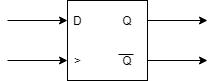
\includegraphics[width=0.2\textwidth]{imagenes/ffd_b.png}
	\caption{Representacion del flip flop}
\end{figure}

\begin{table}[h]
\begin{center}
\begin{tabular}{|l|l|l|}
\hline
clk& D & Q\\
\hline \hline
$\uparrow$ & X & X \\ \hline
$\downarrow$ &X  &$Q_{n-1}$ \\ \hline
\end{tabular}
\caption{Tabla de verdad flip flop d} 
\end{center}
\end{table}

\subsection{Circuito lógico}
Una posible implementación del flip flop d es la siguiente:
\begin{figure}[H]	
	\centering
	
\includegraphics[width=0.5\textwidth]{imagenes/ffd_cd.png}
	\caption{Circuito digital del flip flop d}
\end{figure}
\subsection{Implementación}
Se implementó el circuito indicado en la sección anterior con compuertas lógicas NAND. Para ellos se utilizó el encapsulado 74HC00.
\subsubsection{Medición}
Del circuito previamente mencionado, se midió el tiempo de establecimiento, el rise time y el fall time. 

\begin{table}[h]
\begin{center}
\begin{tabular}{|l|l|l|l|l|}
\hline
clk& D & $Q_{n-1}$ & $Q_n$ &Tiempo de establecimiento\\
\hline \hline
$\uparrow$ &0& 1&0&$25.2 n s$  \\ \hline
$\uparrow$ &1&0&1&$29 n s$  \\ \hline
\end{tabular}
\caption{Resultados,tiempo de establecimiento.} 
\end{center}
\end{table}

\begin{table}[h]
\begin{center}
\begin{tabular}{|l|l|}
\hline
Rise time& Fall time \\
\hline \hline
$45 n s$  & $49.6 n s$ \\ \hline
\end{tabular}
\caption{Resultados, rise time y fall time.} 
\end{center}
\end{table}

Para realizar la comparación se eligió el integrado comercial 74hc74 de la hoja de datos
\footnote{Mouser.com. (2018). [online] Available at: http://www.mouser.com/ds/2/308/74HC74-108792.pdf [Accessed 14 Oct. 2018].}
 Obtuvimos los siguientes tiempos:

\begin{table}[H]
\begin{center}
\begin{tabular}{|l|l|l|l|l|}
\hline
clk& D & $Q_{n-1}$ & $Q_n$ &Tiempo de establecimiento\\
\hline \hline
$\uparrow$ &0& 1&0&$13 n s$  \\ \hline
$\uparrow$ &1&0&1&$18 n s$  \\ \hline
\end{tabular}
\caption{Datasheet,tiempo de establecimiento.} 
\end{center}
\end{table}

\begin{table}[H]
\begin{center}
\begin{tabular}{|l|l|}
\hline
Rise time& Fall time \\
\hline \hline
$<400 n s$  & $<400 n s$ \\ \hline
\end{tabular}
\caption{Datasheet, rise time y fall time.} 
\end{center}
\end{table}

Como se puede observar los tiempos de propagación del flip flop comercial son menores al que se implementó, Esto se puede suponer a que el comercial hace un uso eficiente de los transistores.

\section{Latch SR}

\subsection{Funcionamiento}
El latch SR, posee tres entradas. Una de clock, para poder sincronizar, otra de set (pone la salida a HIGH) y de reset (salida en LOW).
\begin{figure}[H]	
	\centering
	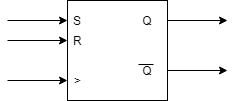
\includegraphics[width=0.2\textwidth]{imagenes/lsr_b.png}
	\caption{Representacion dellatch}
\end{figure}

\begin{table}[h]
\begin{center}
\begin{tabular}{|l|l|l|l|}
\hline
clk&S & R & Q\\
\hline \hline
$\uparrow$ & 0 & 0 & $Q_{n-1}$ \\ \hline
$\uparrow$ & 0 & 1 &0 \\ \hline
$\uparrow$ & 1 & 0 & 1 \\ \hline
$\uparrow$ & 1 &1 & Indeterminado \\ \hline

\end{tabular}
\caption{Tabla de verdad latch  SR} 
\end{center}
\end{table}

\subsection{Circuito lógico}
Una posible implementación del latch SR es la siguiente:
\begin{figure}[H]	
	\centering
	
\includegraphics[width=0.5\textwidth]{imagenes/lsr_cd.png}
	\caption{Circuito digital del flip flop d}
\end{figure}

\subsection{Implementación}
Se implementó el circuito indicado en la sección anterior con compuertas lógicas NAND, las compuertas NOR tambien se implenetaron con NANDS. Para ellos se utilizó el encapsulado 74HC00.
\subsubsection{Medición}
Del circuito previamente mencionado, se midió el tiempo de establecimiento, el rise time y el fall time. 

\begin{table}[h]
\begin{center}
\begin{tabular}{|l|l|l|l|l|l|}
\hline
clk& R&S & $Q_{n-1}$ & $Q_n$ &Tiempo de establecimiento\\
\hline \hline
$\uparrow$ &0 & 1 &0&1&$21.6 n s$  \\ \hline
$\uparrow$ &1 & 0 &1&0&$14 n s$  \\ \hline

\end{tabular}
\caption{Resultados,tiempo de establecimiento.} 
\end{center}
\end{table}

\begin{table}[h]
\begin{center}
\begin{tabular}{|l|l|}
\hline
Rise time& Fall time \\
\hline \hline
$21.6 n s$  & $14 n s$ \\ \hline
\end{tabular}
\caption{Resultados, rise time y fall time.} 
\end{center}
\end{table}

Para realizar la comparación se eligió el integrado comercial 74hc279 de la hoja de datos
\footnote{Noel.feld.cvut.cz. (2018). [online] Available at: http://noel.feld.cvut.cz/hw/st/1937.pdf [Accessed 14 Oct. 2018].}
 Obtuvimos los siguientes tiempos:

\begin{table}[H]
\begin{center}
\begin{tabular}{|l|l|l|l|l|}
\hline
clk& D & $Q_{n-1}$ & $Q_n$ &Tiempo de establecimiento\\
\hline \hline
$\uparrow$ &0& 1&0&$20n s$  \\ \hline
$\uparrow$ &1&0&1&$13 n s$  \\ \hline
\end{tabular}
\caption{Datasheet,tiempo de establecimiento.} 
\end{center}
\end{table}

\begin{table}[H]
\begin{center}
\begin{tabular}{|l|l|}
\hline
Rise time& Fall time \\
\hline \hline
$<400 n s$  & $<400 n s$ \\ \hline
\end{tabular}
\caption{Datasheet, rise time y fall time.} 
\end{center}
\end{table}






\end{document}
